\section{Séance 4 - Déphasage et linéarité}

\subsection{Objectif}

L'objectif de cette séance est de déterminer quel déphasage entre les signaux 
$U_{exc}$ et $U_{p}$ génère la réponse la plus linéaire en fonction de la distance.

\subsection{Théorie}

Le déphasage joue un rôle crucial dans le fonctionnement du capteur, car il impacte directement 
ses performances. Un déphasage inapproprié pourrait entraîner une réponse non linéaire du capteur,
 rendant ainsi les valeurs mesurées difficiles à interpréter, voire inutilisables. 
 
 Afin d'assurer une interprétation fiable des données et une exploitation optimale des mesures,
  il est essentiel de minimiser l'erreur de linéarité. Cette réduction contribue directement à 
  l'amélioration des performances globales du capteur.


\subsection{Méthode}

\begin{itemize}
    \item Montage : 
    \begin{enumerate}
    \item Alimenter le PCB à -12 et 12 V;
    \item Le jumper J3 doit être monté entre 1 et 2; 
    \item Alimenter $U_{exc}$ avec un signal carré 0-5 V;
    \item Alimenter $U_{p}$ avec un signal carré 0-5 V;
    \item Brancher la sortie $U_{out}$ au multimètre de table pour plus de précision.
\end{enumerate}


\begin{figure}[H]
    \centering
    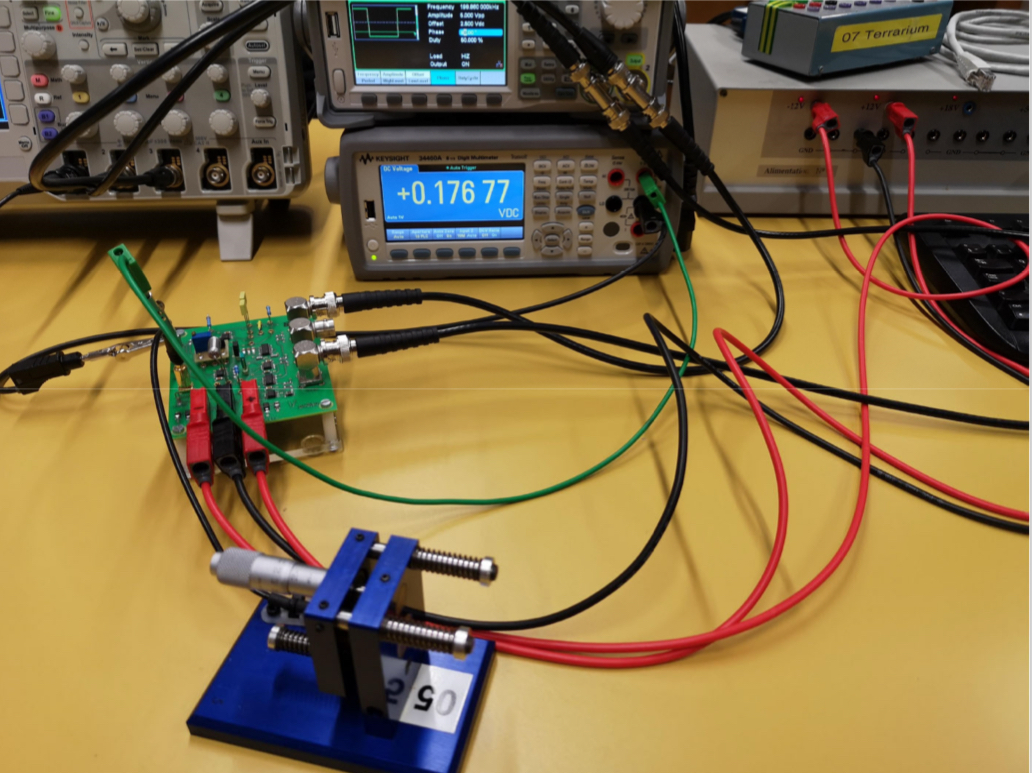
\includegraphics[width=6cm]{Images/Seance4/MT4.jpg}
    \caption{Montage - Séance 4  }
    \label{fig:lum}
\end{figure}
\item Mesures :
\begin{enumerate}
    \item Positionner le capteur à 0.5 mm;
    \item Mesurer la tension $U_{out}$ obtenue pour chaque déphasage entre $U_{exc}$ et $U_{mod}$
    de 0° à 180° par pas de 30°;
    \item Répéter l'opération 2 pour chaque distance par pas de 0.05 mm jusqu'à 0.9 mm.
\end{enumerate}
\end{itemize}

\subsection{Résultats}


Voici les différentes valeurs mesurées permettant de visualiser la réponse du capteur aux différents
déphasages et positions :

\begin{table}[H]
    \centering
    \begin{tabular}{|c|ccccccc|}
    \hline
    \textbf{}                  & \multicolumn{7}{c|}{\textbf{Déphasage {[}°{]}}}                                                                                                                                                                                 \\ \hline
    \textbf{Distance {[}mm{]}} & \multicolumn{1}{c|}{\textbf{0}} & \multicolumn{1}{c|}{\textbf{30}} & \multicolumn{1}{c|}{\textbf{60}} & \multicolumn{1}{c|}{\textbf{90}} & \multicolumn{1}{c|}{\textbf{120}} & \multicolumn{1}{c|}{\textbf{150}} & \textbf{180} \\ \hline
    \textbf{0.5}               & \multicolumn{1}{c|}{263.24}     & \multicolumn{1}{c|}{424.82}      & \multicolumn{1}{c|}{484.9}       & \multicolumn{1}{c|}{413.9}       & \multicolumn{1}{c|}{225.17}       & \multicolumn{1}{c|}{-29.66}       & -269.25      \\ \hline
    \textbf{0.55}              & \multicolumn{1}{c|}{277.65}     & \multicolumn{1}{c|}{444.38}      & \multicolumn{1}{c|}{504.05}      & \multicolumn{1}{c|}{427.65}      & \multicolumn{1}{c|}{230.19}       & \multicolumn{1}{c|}{-34.88}       & -283.6       \\ \hline
    \textbf{0.6}               & \multicolumn{1}{c|}{292.83}     & \multicolumn{1}{c|}{464.76}      & \multicolumn{1}{c|}{528.86}      & \multicolumn{1}{c|}{441.71}      & \multicolumn{1}{c|}{235.16}       & \multicolumn{1}{c|}{-40.49}       & -298.9       \\ \hline
    \textbf{0.65}              & \multicolumn{1}{c|}{307.48}     & \multicolumn{1}{c|}{484.06}      & \multicolumn{1}{c|}{542.34}      & \multicolumn{1}{c|}{454.6}       & \multicolumn{1}{c|}{239.39}       & \multicolumn{1}{c|}{-46.32}       & -313.7       \\ \hline
    \textbf{0.7}               & \multicolumn{1}{c|}{323.25}     & \multicolumn{1}{c|}{504.52}      & \multicolumn{1}{c|}{561.7}       & \multicolumn{1}{c|}{467.82}      & \multicolumn{1}{c|}{243.46}       & \multicolumn{1}{c|}{-53}          & -329.57      \\ \hline
    \textbf{0.75}              & \multicolumn{1}{c|}{337.95}     & \multicolumn{1}{c|}{523.13}      & \multicolumn{1}{c|}{578.93}      & \multicolumn{1}{c|}{479.2}       & \multicolumn{1}{c|}{246.25}       & \multicolumn{1}{c|}{-59.61}       & -344.45      \\ \hline
    \textbf{0.8}               & \multicolumn{1}{c|}{353.22}     & \multicolumn{1}{c|}{542.29}      & \multicolumn{1}{c|}{596.52}      & \multicolumn{1}{c|}{490.75}      & \multicolumn{1}{c|}{249.12}       & \multicolumn{1}{c|}{-66.53}       & -359.78      \\ \hline
    \textbf{0.85}              & \multicolumn{1}{c|}{368.82}     & \multicolumn{1}{c|}{561.63}      & \multicolumn{1}{c|}{614.06}      & \multicolumn{1}{c|}{502.05}      & \multicolumn{1}{c|}{251.64}       & \multicolumn{1}{c|}{-73.82}       & -375.41      \\ \hline
    \textbf{0.9}               & \multicolumn{1}{c|}{383.79}     & \multicolumn{1}{c|}{579.89}      & \multicolumn{1}{c|}{630.41}      & \multicolumn{1}{c|}{512.35}      & \multicolumn{1}{c|}{253.66}       & \multicolumn{1}{c|}{-81.05}       & -390.45      \\ \hline
    \end{tabular}
    \caption{Tension aux différents déphasages et distances}
    \end{table}


    \insererfigure{Images/Seance4/Rep.png}{9cm}{Réponse du capteur - séance 4}{Sensibi}

L'erreur de linéarité a ensuite été tracée :  

    \insererfigure{Images/Seance4/Err.png}{9cm}{Régressions selon le déphasage}{lin}

    Minimum à 0° (0.4706 \%)

    \subsection{Analyse}

    Les valeurs présentées dans la figure \ref{fig: Sensibi} semblent cohérentes, avec des courbes qui, 
    visuellement, apparaissent globalement linéaires.

    La courbe d'erreur de linéarité \ref{fig: lin} confirme une très bonne linéarité des courbes, 
    avec une non-linéarité maximale de 7,5 \% observée à 120°, tandis que la non-linéarité la plus 
    faible, de 0,47 \%, est relevée à 0°. \\
    
    Cependant, \textbf{l'allure} de la non-linéarité diffère de celle attendue. En effet, pour ce type de 
    capteur, il est généralement supposé que la linéarité maximale se situe dans une plage de 
    déphasage comprise entre 80° et 130°.\\ 

    Cela soulève donc les interrogations suivantes quant à la validité des résultats obtenus : 

    \begin{itemize} \item Les valeurs semblent similaires pour 0° et 180°, ce qui pourrait
         s'expliquer par la $\pi$-périodicité du déphasage. Bien que cela puisse sembler inhabituel, 
         y trouver un minimum n'est pas nécessairement incorrect ;
         \item Une erreur de montage pourrait être en cause : un problème lié à une résistance, 
         un condensateur ou un fil mal connecté ; 
         \item Une mesure aurait pu être effectuée sur une sortie incorrecte de la carte (par exemple $U_{mult}$); 
         \item Un défaut du fil du capteur est également envisageable, bien que peu probable compte 
         tenu de la forte linéarité des résultats. 
        \end{itemize}

        \subsection{Conclusion}

        Les différentes mesures ont pu être réalisées lors de cette 4$^{\text{ème}}$ séance. Ceux-ci ont
        permis de déterminer une non-linéarité minimale du système de 0.47 \% à 0°. Cependant,
        ces résultats ont été jugés très incertains. La prochaine manipulation permettra de 
        confirmer cette supposition.  